\documentclass[aspectratio=169, 11pt]{beamer}

%% ── Theme ──────────────────────────────────────────────────────
\usetheme[progressbar=frametitle]{metropolis}

%% ── Packages ───────────────────────────────────────────────────
\usepackage[T1]{fontenc}
\usepackage[utf8]{inputenc}
\usepackage{lmodern}
\usepackage[absolute,overlay]{textpos}
\usepackage{appendixnumberbeamer}
\usepackage{xcolor}
\usepackage{booktabs}
\usepackage{tikz}
\usepackage{hyperref}
\usepackage{xspace}
\usepackage{amsmath,amssymb}
\usetikzlibrary{arrows.meta,positioning,fit,backgrounds,calc}

%% ── Notes ──
\usepackage{pgfpages}
\setbeameroption{hide notes}

%% ── ORNL colors ────────────────────────────────────────────────
\definecolor{ornlgreen}{RGB}{0,121,52}
\definecolor{ornlblack}{RGB}{0,0,0}
\definecolor{ornlgrey}{RGB}{88,88,88}
\definecolor{backgroundgreen}{RGB}{68,126,89}
\definecolor{backgroundgrey}{RGB}{191,191,191}
\definecolor{cerulean}{RGB}{0,122,166}

\setbeamercolor{progress bar}{fg=ornlgreen, bg=ornlgreen!30}
\setbeamercolor{normal text}{fg=ornlblack, bg=white}
\setbeamercolor{frametitle}{fg=ornlblack, bg=white}
\setbeamercolor{structure}{fg=ornlgreen}
\setbeamercolor{itemize item}{fg=ornlgreen}
\setbeamercolor{block title}{fg=white, bg=ornlgreen}
\setbeamercolor{block body}{fg=ornlblack, bg=ornlgreen!8}

\usebackgroundtemplate{%
  
\includegraphics[width=\paperwidth]{style/assets/slide_frame.png}}

\newcommand{\maketitlepage}{%
  {\usebackgroundtemplate{%
     
\includegraphics[angle=0,width=\paperwidth]{style/assets/title_frame.png}}%
   \begin{frame}\titlepage\end{frame}}}
\defbeamertemplate*{title page}{customized}[1][]{%
  \setbeamertemplate{footline}{}
  \textcolor{white}{\Huge \inserttitle}\\[4pt]
  \textcolor{white}{\large \insertsubtitle}\\[14pt]
  \textcolor{white}{\Large \insertauthor}\\[4pt]
  \textcolor{white}{\insertdate}}

\hypersetup{colorlinks=true,linkcolor=blue,urlcolor=cerulean,citecolor=blue}

%% ── Metadata ───────────────────────────────────────────────────
\title{\small AI-Agent Driven Survey and Validated Literature Review for Discovering Solid Breeder Materials}
\subtitle{End-to-End Traceability for Automated Literature Generation}
\author{Jose Tupayachi, Gabe Parker, Xueping Li and Xiao-Ying Yu\textsuperscript{*}}

\institute{
Materials Science and Technology Division\\
\small Research supported by DOE FES
}

\date{
\tiny
ANS TOFE 2026\\
Denver, Colorado\\[4pt]
\scriptsize Research supported by DOE FES
}

\begin{document}

%% ═══════════════════════════════════════════════════════════════
%% 1 — TITLE / ORNL INTRO
%% ═══════════════════════════════════════════════════════════════
\maketitlepage

%% ═══════════════════════════════════════════════════════════════
%% 2 — APPROACH: CURRENT vs OURS
%% ═══════════════════════════════════════════════════════════════
\begin{frame}{Solid Breeders are a Bottleneck for Fusion Energy}
\vspace{4pt}

\begin{columns}[T]
  \begin{column}{0.48\textwidth}
    \centering\textbf{\color{ornlgrey}Current Approaches}\\[10pt]
    \footnotesize
    \begin{itemize}\setlength\itemsep{6pt}
      \item Analyze papers and databases individually
      \item Limited claim-level verification
      \item Static LLM prompts cannot explore research questions in depth
      \item Focus on prediction, not review generation
    \end{itemize}
  \end{column}
  \begin{column}{0.04\textwidth}\centering
    \rule{0.5pt}{4cm}
  \end{column}
  \begin{column}{0.46\textwidth}
    \centering\textbf{\color{ornlgreen}Our Approach}\\[10pt]
    \footnotesize
    \begin{itemize}\setlength\itemsep{6pt}
      \item Integrate multimodal information (incl.\ ontologies)
      \item Verifies every sentence
      \item Produces traceable review manuscripts automatically
      \item Graph-based approach enables deeper exploration of research questions
    \end{itemize}
  \end{column}
\end{columns}

\vfill
{\scriptsize\color{ornlgrey}
\textbf{References:}\;
\tiny
Zhou \emph{et al.}, \emph{Int.\ Dent.\ J.} 2026 \href{https://doi.org/10.1016/j.identj.2025.07.013}{doi:10.1016/j.identj.2025.07.013}~$\circ$
Tasdemir, \emph{J.\ Alloys Metall.\ Syst.} 2026 \href{https://doi.org/10.1016/j.jalmes.2025.100192}{doi:10.1016/j.jalmes.2025.100192}~$\circ$
Tang \emph{et al.} (MatterChat), \emph{Nat.\ Mach.\ Intell.} 2026 \href{https://doi.org/10.1038/s42256-025-01065-z}{doi:10.1038/s42256-025-01065-z}~$\circ$
Zhang \emph{et al.}, \emph{Adv.\ Funct.\ Mater.} 2026 \href{https://doi.org/10.1002/adfm.202508472}{doi:10.1002/adfm.202508472}.\par}
\end{frame}

%% ═══════════════════════════════════════════════════════════════
%% 3 — APPROACH: SIX-STAGE PIPELINE + LANGGRAPH ZOOM
%% ═══════════════════════════════════════════════════════════════
\begin{frame}{Six Stages End-to-End | Writing Stage Expands Into a 5-Agent LangGraph With Shared State}
\centering
%% ── Top: six-stage pipeline ────────────────────────────────────
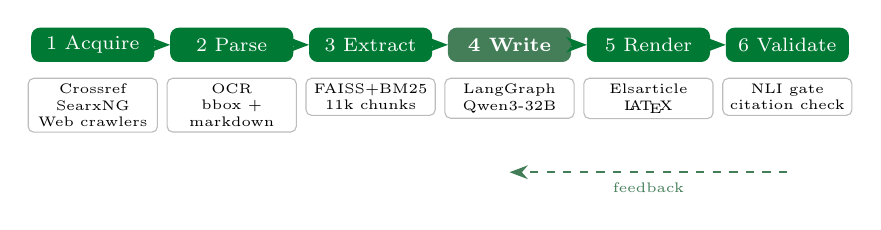
\begin{tikzpicture}[font=\scriptsize,
  stage/.style={draw=ornlgreen,fill=ornlgreen,text=white,rounded corners=3pt,
                minimum height=1.2em,minimum width=1.55cm,inner sep=2pt,align=center},
  sub/.style={draw=ornlgrey!40,fill=white,rounded corners=2pt,
              inner sep=2pt,align=center,font=\tiny,text width=1.50cm,
              text=ornlblack},
  arr/.style={-Stealth,line width=1.0pt,ornlgreen}]
  \node[stage](s1){1 Acquire};
  \node[stage,right=0.20cm of s1](s2){2 Parse};
  \node[stage,right=0.20cm of s2](s3){3 Extract};
  \node[stage,right=0.20cm of s3,fill=backgroundgreen,draw=backgroundgreen](s4){\textbf{4 Write}};
  \node[stage,right=0.20cm of s4](s5){5 Render};
  \node[stage,right=0.20cm of s5](s6){6 Validate};
  \foreach \a/\b in {s1/s2,s2/s3,s3/s4,s4/s5,s5/s6}{\draw[arr](\a)--(\b);}
  \node[sub,below=0.20cm of s1]{Crossref\\SearxNG \\ Web crawlers};
  \node[sub,below=0.20cm of s2]{OCR\\bbox + markdown};
  \node[sub,below=0.20cm of s3]{FAISS+BM25\\11k chunks};
  \node[sub,below=0.20cm of s4]{LangGraph\\Qwen3-32B};
  \node[sub,below=0.20cm of s5]{Elsarticle\\ \LaTeX};
  \node[sub,below=0.20cm of s6]{NLI gate\\citation check};
  \draw[dashed,-Stealth,backgroundgreen,thick]
    ([yshift=-1.4cm]s6.south)--
    node[below,font=\tiny,text=backgroundgreen]{feedback}
    ([yshift=-1.4cm]s4.south);
\end{tikzpicture}\\[2pt]
%% ── Connecting arrow ───────────────────────────────────────────
{\large\textbf{\color{backgroundgreen}$\Downarrow$ zoom into Stage 4 (Write)}}\\[2pt]
%% ── Bottom: LangGraph 5-agent diagram ──────────────────────────
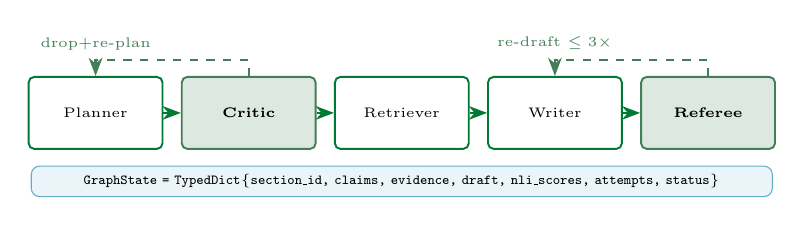
\begin{tikzpicture}[font=\tiny,
  box/.style={draw=ornlgreen,fill=white,rounded corners=2pt,
              minimum height=2.6em,minimum width=1.7cm,
              inner sep=2pt,align=center,text=ornlblack,line width=0.7pt},
  gate/.style={draw=backgroundgreen,fill=backgroundgreen!18,rounded corners=2pt,
               minimum height=2.6em,minimum width=1.7cm,
               inner sep=2pt,align=center,text=ornlblack,
               font=\tiny\bfseries,line width=0.7pt},
  state/.style={draw=cerulean!60,fill=cerulean!8,rounded corners=3pt,
                inner sep=3pt,align=center,text=ornlblack,
                font=\tiny\ttfamily,text width=9.2cm},
  arr/.style={-Stealth,ornlgreen,thick}]
  \node[box](plan){Planner};
  \node[gate,right=0.22cm of plan](crit){Critic};
  \node[box,right=0.22cm of crit](ret){Retriever};
  \node[box,right=0.22cm of ret](write){Writer};
  \node[gate,right=0.22cm of write](ref){Referee};
  \draw[arr](plan)--(crit);\draw[arr](crit)--(ret);
  \draw[arr](ret)--(write);\draw[arr](write)--(ref);
  \draw[-Stealth,dashed,backgroundgreen,thick]
    (crit.north)--++(0,0.20)-|node[above,font=\tiny]{drop+re-plan}(plan.north);
  \draw[-Stealth,dashed,backgroundgreen,thick]
    (ref.north)--++(0,0.20)-|node[above,font=\tiny]{re-draft $\leq 3\times$}(write.north);
  \node[state,below=0.20cm of ret]{%
    GraphState = TypedDict\{section\_id, claims, evidence, draft,
    nli\_scores, attempts, status\}};
\end{tikzpicture}\\[2pt]
{\scriptsize\color{ornlgreen}\textbf{Why a graph:} Breaks broad scientific questions into focused sub-questions; shared state records sources and decisions for per-claim traceability.}
\end{frame}

\end{document}
